\documentclass[aspectratio=169,10pt]{beamer}

\usetheme{Madrid}
\usecolortheme{seahorse}
\setbeamertemplate{footline}[frame number]

%──────────────────────────────────────────────────────────────
% Packages
%──────────────────────────────────────────────────────────────
\usepackage{amsmath,amssymb,amsfonts}
\usepackage{mathtools}
\usepackage{bm}
\usepackage{booktabs}
\usepackage{graphicx}
\usepackage{listings}
\usepackage{xcolor}
\usepackage{tikz}
\usepackage{array}
\usepackage{multicol}

\graphicspath{{figures/}}

%──────────────────────────────────────────────────────────────
% Listings: Python style
%──────────────────────────────────────────────────────────────
\lstdefinestyle{python}{
  language=Python,
  basicstyle=\ttfamily\scriptsize,
  numbers=left,
  numberstyle=\tiny\color{gray},
  frame=single,
  backgroundcolor=\color{gray!7},
  keywordstyle=\color{blue}\bfseries,
  commentstyle=\color{green!60!black},
  stringstyle=\color{red!70!black},
  breaklines=true,
  tabsize=4,
  showstringspaces=false,
  captionpos=b,
}
\lstset{style=python}

%──────────────────────────────────────────────────────────────
% Convenience macros
%──────────────────────────────────────────────────────────────
\newcommand{\vx}{\mathbf{x}}
\newcommand{\vg}{\mathbf{g}}
\newcommand{\vd}{\mathbf{d}}
\newcommand{\vv}{\mathbf{v}}
\newcommand{\vs}{\mathbf{s}}
\newcommand{\vu}{\mathbf{u}}
\newcommand{\vb}{\mathbf{b}}
\newcommand{\mA}{\mathbf{A}}
\newcommand{\R}{\mathbb{R}}
\newcommand{\norm}[1]{\left\|#1\right\|}

%──────────────────────────────────────────────────────────────
% Title
%──────────────────────────────────────────────────────────────
\title[Ch.\ 5: First-Order Methods]{Chapter 5: First-Order Methods}
\subtitle{Algorithms for Optimization, 2nd ed.\ (2026)\\
          Kochenderfer \& Wheeler}
\author{Lecture Notes}
\date{\today}

\begin{document}

%──────────────────────────────────────────────────────────────
\begin{frame}
  \titlepage
\end{frame}

%──────────────────────────────────────────────────────────────
\begin{frame}{Table of Contents}
  \tableofcontents
\end{frame}

%==============================================================
\section{Introduction to First-Order Methods}
%==============================================================

\begin{frame}{What Are First-Order Methods?}
  \begin{columns}[T]
    \column{0.52\textwidth}
      \begin{block}{Definition}
        \textbf{First-order methods} use gradient information
        $\nabla f(\vx)$ to select a descent direction.
      \end{block}

      \vspace{0.4em}
      \textbf{Why gradient information?}
      \begin{itemize}
        \item Gradient points in the direction of \emph{steepest ascent}
        \item Opposite direction is the direction of \emph{steepest descent}
        \item Computing $\nabla f$ costs $O(n)$ for most functions (vs.\
              $O(n^2)$ for Hessian)
        \item Scalable to high-dimensional problems (e.g.\ deep learning)
      \end{itemize}

      \vspace{0.4em}
      \begin{alertblock}{Requirement}
        $f$ must be \emph{differentiable} (or sub-differentiable for
        non-smooth $f$ — see Appendix C.5).
      \end{alertblock}

    \column{0.45\textwidth}
      \begin{block}{Chapter Roadmap}
        \footnotesize
        \begin{enumerate}
          \item Gradient Descent (steepest descent)
          \item Conjugate Gradient Method
          \item Momentum (Heavy Ball)
          \item Nesterov Momentum
          \item AdaGrad
          \item RMSProp
          \item Adadelta
          \item Adam
          \item Hypergradient Descent
        \end{enumerate}
      \end{block}
  \end{columns}
\end{frame}

%==============================================================
\section{5.1 Gradient Descent}
%==============================================================

\begin{frame}{5.1 Gradient Descent — Motivation}
  \begin{columns}[T]
    \column{0.55\textwidth}
      Define the gradient at the $k$-th iterate $\vx^{(k)}$:
      \begin{block}{Gradient Notation (Eq.\ 5.1)}
        \[
          \vg^{(k)} = \nabla f\!\left(\vx^{(k)}\right)
        \]
        \begin{itemize}
          \item $\vg^{(k)} \in \R^n$: partial derivatives at $\vx^{(k)}$
        \end{itemize}
      \end{block}

      \textbf{First-order Taylor approximation} about $\vx^{(k)}$:
      \begin{block}{Linear Approximation (Eq.\ 5.2)}
        \[
          f\!\left(\vx^{(k)}+\alpha\vd\right)
          \approx f\!\left(\vx^{(k)}\right) + \alpha\,\vd^\top\vg^{(k)}
        \]
        \begin{itemize}
          \item $\alpha$: step factor (learning rate)
          \item $\vd$: unit descent direction ($\norm{\vd}=1$)
        \end{itemize}
      \end{block}

      \textbf{Minimizing} over $\vd$ subject to $\norm{\vd}=1$
      gives the \emph{steepest descent} direction:
      \begin{block}{Steepest Descent Direction (Eq.\ 5.3)}
        \[
          \vd^{(k)} = -\frac{\vg^{(k)}}{\norm{\vg^{(k)}}}
        \]
      \end{block}

    \column{0.42\textwidth}
      \textbf{Update rule}:
      \[
        \vx^{(k+1)} = \vx^{(k)} - \alpha\,\vg^{(k)}
      \]
      (many implementations skip normalisation; then $\alpha$ is not
      the step \emph{length})

      \vspace{0.5em}
      \textbf{Key insight}: moving \emph{opposite} the gradient
      decreases $f$ locally.

      \vspace{0.5em}
      \begin{alertblock}{Note (L\textsubscript{2} norm)}
        Using the $L_2$ norm gives steepest descent.
        Using the $L_1$ norm gives \emph{coordinate descent}.
      \end{alertblock}
  \end{columns}
\end{frame}

\begin{frame}[fragile]{5.1 Gradient Descent — Algorithm and Python Code}
  \begin{columns}[T]
    \column{0.48\textwidth}
      \begin{block}{Algorithm: Gradient Descent}
        \footnotesize
        \textbf{Input}: $f$, $\nabla f$, initial $\vx^{(1)}$, step $\alpha$,
                        iterations $T$\\[3pt]
        \textbf{For} $k = 1, 2, \dots, T$:
        \begin{enumerate}
          \item Compute $\vg^{(k)} = \nabla f(\vx^{(k)})$
          \item Normalise: $\vd^{(k)} = -\vg^{(k)}/\norm{\vg^{(k)}}$
          \item Update: $\vx^{(k+1)} = \vx^{(k)} + \alpha\,\vd^{(k)}$
        \end{enumerate}
        \textbf{Return} $\vx^{(T+1)}$\\[3pt]
        \textit{Cost per iteration}: 1 gradient evaluation, $O(n)$
      \end{block}

      \vspace{0.5em}
      \textbf{Convergence} (for $L$-smooth, $\mu$-strongly convex $f$):
      \[
        \norm{\vx^{(k)}-\vx^*}^2 \le
        \left(1 - \frac{\mu}{L}\right)^k \norm{\vx^{(1)}-\vx^*}^2
      \]
      Linear convergence rate $\kappa = \mu/L$ (condition number).

    \column{0.50\textwidth}
      \begin{lstlisting}[caption={Gradient Descent (Python/NumPy)}]
import numpy as np

def gradient_descent(f, grad_f, x, alpha,
                     n_iter=100, normalize=True):
    """
    f        : objective function
    grad_f   : gradient of f
    x        : initial point (1D numpy array)
    alpha    : step factor
    normalize: use unit step direction
    """
    path = [x.copy()]
    for _ in range(n_iter):
        g = grad_f(x)
        if normalize:
            d = -g / (np.linalg.norm(g) + 1e-15)
        else:
            d = -g          # unnormalized
        x = x + alpha * d
        path.append(x.copy())
    return x, np.array(path)

# Example: f(x) = x1^2 * x2
f     = lambda x: x[0]**2 * x[1]
gradf = lambda x: np.array([2*x[0]*x[1], x[0]**2])

x0 = np.array([1.0, 2.0])
x_opt, path = gradient_descent(f, gradf, x0, alpha=0.1)
\end{lstlisting}
  \end{columns}
\end{frame}

\begin{frame}{5.1 Gradient Descent — Paths and Numerical Example}
  \begin{columns}[T]
    \column{0.48\textwidth}
      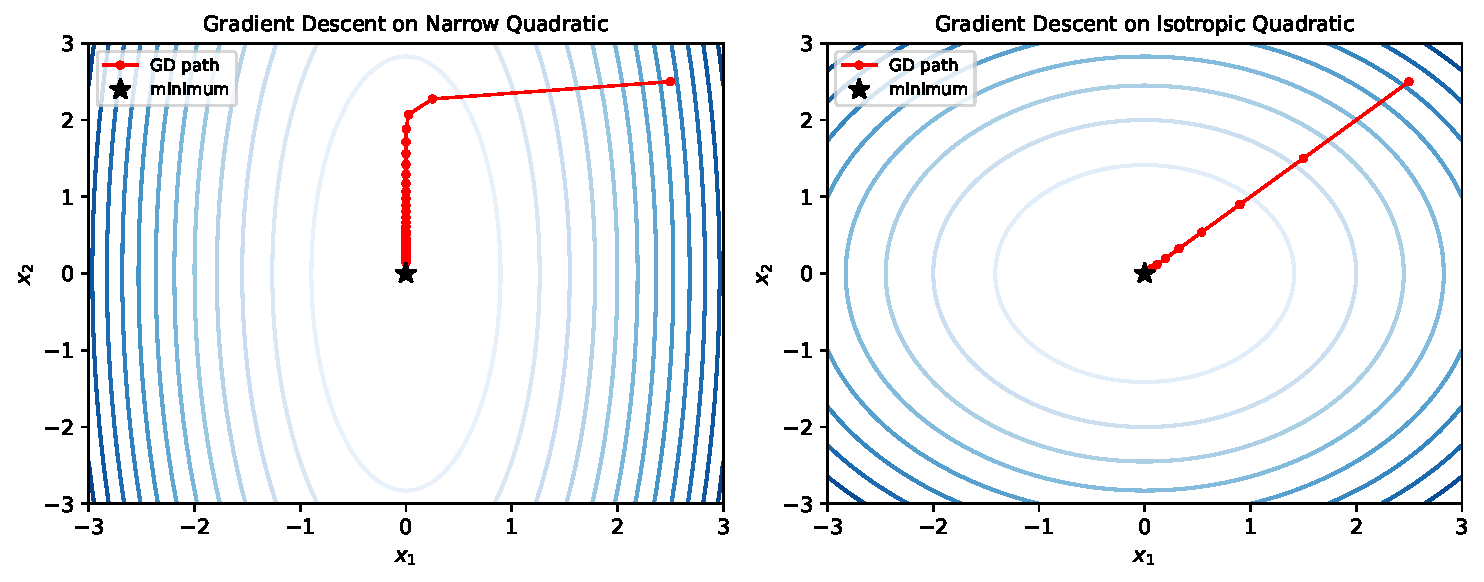
\includegraphics[width=\textwidth]{gradient_descent_paths}

      \footnotesize
      \textit{Left}: zigzag on ill-conditioned quadratic.
      \textit{Right}: smooth convergence on isotropic quadratic.

    \column{0.50\textwidth}
      \textbf{Numerical Example}: $f(\vx) = x_1 x_2^2$

      At $\vx^{(k)} = [1, 2]$, $\alpha = 0.1$ (normalised):
      \[
        \nabla f = [x_2^2,\; 2x_1 x_2]
                = [4,\; 4]
      \]
      \[
        \vd^{(k)} = -\frac{[4, 4]}{\sqrt{32}}
                  = \left[-\frac{1}{\sqrt{2}},\, -\frac{1}{\sqrt{2}}\right]
      \]
      \[
        \vx^{(k+1)} = [1, 2] + 0.1\left[-\tfrac{1}{\sqrt{2}},
                                         -\tfrac{1}{\sqrt{2}}\right]
                    \approx [0.929,\, 1.929]
      \]

      \vspace{0.5em}
      \textbf{Weakness}: may zig-zag in narrow valleys. The step
      size $\alpha$ must be tuned carefully.

      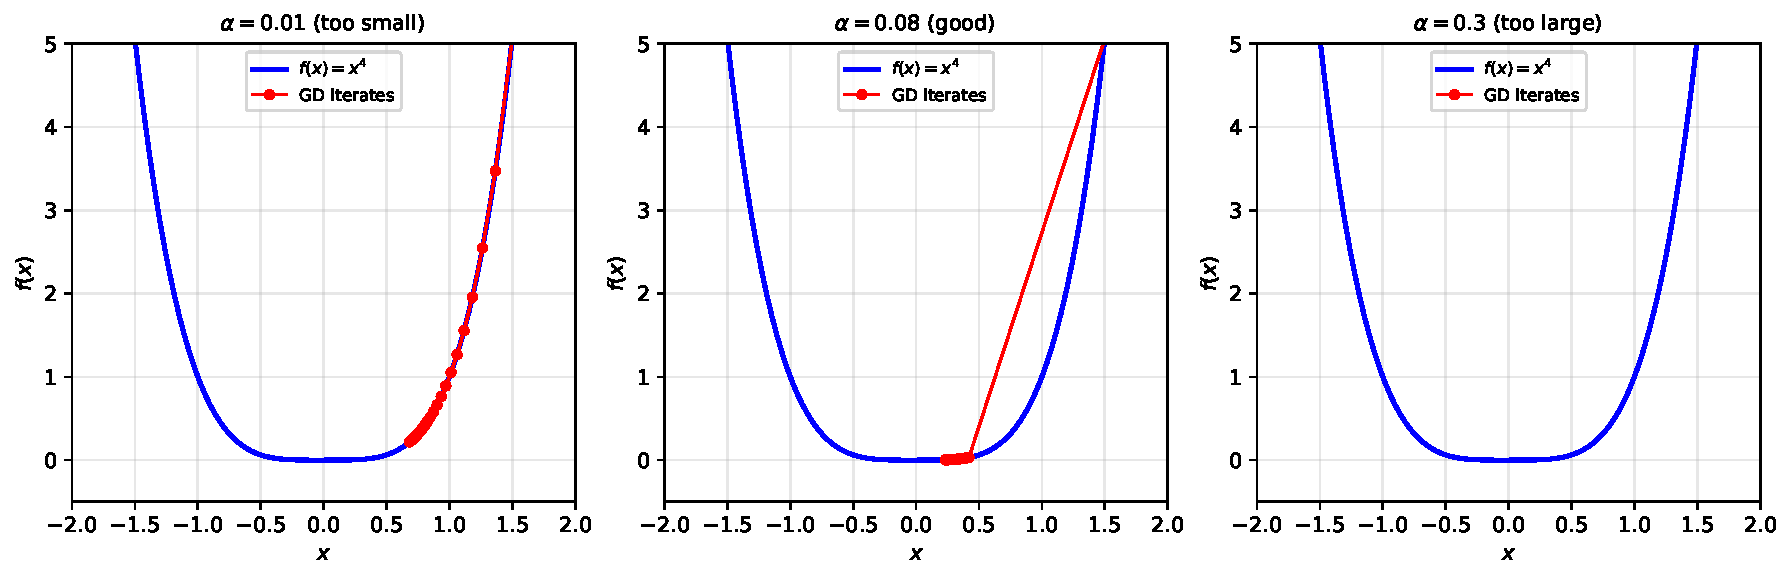
\includegraphics[width=0.9\textwidth]{step_size_effect}
      \footnotesize Too small $\Rightarrow$ slow; too large $\Rightarrow$ diverges.
  \end{columns}
\end{frame}

%==============================================================
\section{5.2 Conjugate Gradient Method}
%==============================================================

\begin{frame}{5.2 Conjugate Gradient — Motivation}
  \begin{columns}[T]
    \column{0.52\textwidth}
      \textbf{Problem with gradient descent}: on narrow valleys,
      successive gradients are \emph{nearly orthogonal} $\Rightarrow$
      slow zigzagging.

      \vspace{0.4em}
      \textbf{Conjugate gradient (CG)} borrows from exact solvers for
      quadratic objectives:
      \begin{block}{Quadratic Objective (Eq.\ 5.8)}
        \[
          \min_{\vx}\; \tfrac{1}{2}\vx^\top\mA\vx + \vb^\top\vx + c
        \]
        $\mA$ symmetric positive definite $\Rightarrow$ unique minimum.
      \end{block}

      \begin{block}{Key Property: Conjugacy (Eq.\ 5.9)}
        Directions $\vd^{(1)}, \dots, \vd^{(n)} \ne \mathbf{0}$
        are \textbf{mutually conjugate} w.r.t.\ $\mA$ if:
        \[
          \vd^{(i)\top}\mA\,\vd^{(j)} = 0 \quad \text{for all } i \ne j
        \]
      \end{block}

      \textbf{Result}: CG optimises an $n$-dimensional quadratic in
      exactly $n$ steps!

    \column{0.46\textwidth}
      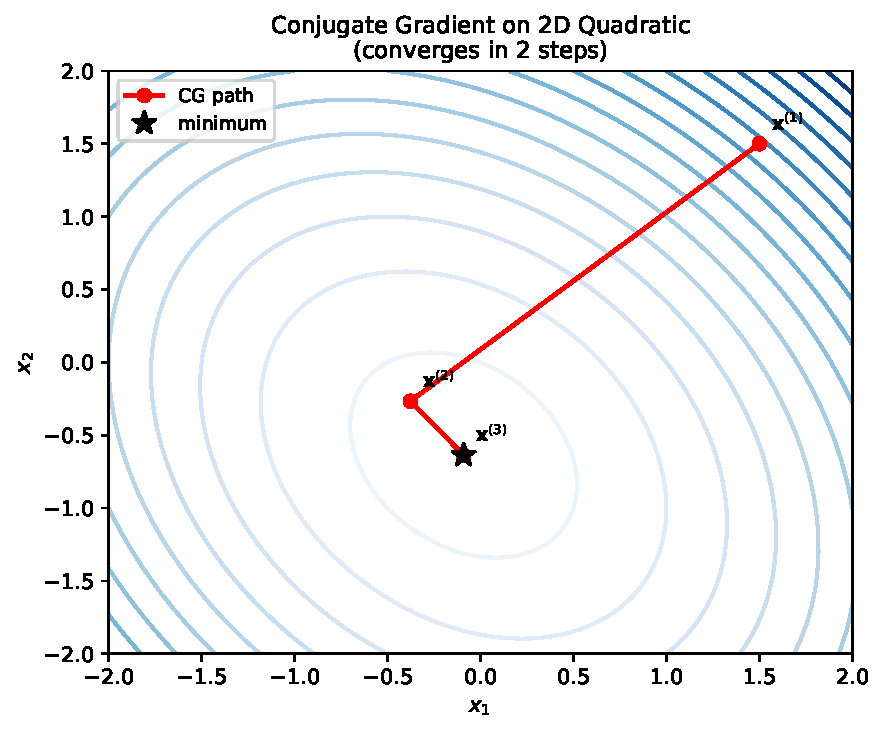
\includegraphics[width=\textwidth]{conjugate_gradient}

      \footnotesize Conjugate gradient converges in $n=2$ steps
      on a 2-D quadratic. Note: the search directions are \emph{not}
      orthogonal in general.
  \end{columns}
\end{frame}

\begin{frame}[allowframebreaks]{5.2 Conjugate Gradient — Update Rules}
  \textbf{Step 1 — initialise} with steepest descent:
  \[
    \vd^{(1)} = -\vg^{(1)} \tag{5.10}
  \]

  \textbf{Step 2 — exact line search} (for quadratic $f$, Example 5.1):
  \[
    \alpha = -\frac{\vd^\top(\mA\vx + \vb)}{\vd^\top\mA\vd}
           = -\frac{\vd^\top\vg}{\vd^\top\mA\vd}
  \]
  \[
    \vx^{(2)} = \vx^{(1)} + \alpha^{(1)}\vd^{(1)} \tag{5.11}
  \]

  \textbf{Step $k>1$ — update direction} (Eq.\ 5.12):
  \[
    \vd^{(k)} = -\vg^{(k)} + \beta^{(k)}\vd^{(k-1)}
  \]

  \textbf{Optimal $\beta^{(k)}$} (when $\mA$ is known, Eq.\ 5.16):
  \[
    \beta^{(k)} = \frac{\vg^{(k)\top}\mA\,\vd^{(k-1)}}{\vd^{(k-1)\top}\mA\,\vd^{(k-1)}}
  \]

  \framebreak

  \textbf{For general (non-quadratic) functions}: several approximations
  that do \emph{not} require $\mA$:

  \begin{block}{Fletcher--Reeves update (Eq.\ 5.17)}
    \[
      \beta^{(k)}_{\mathrm{FR}} = \frac{\vg^{(k)\top}\vg^{(k)}}
                                        {\vg^{(k-1)\top}\vg^{(k-1)}}
    \]
    Ratio of squared norms of successive gradients.
  \end{block}

  \begin{block}{Polak--Ribi\`{e}re update (Eq.\ 5.18)}
    \[
      \beta^{(k)}_{\mathrm{PR}}
      = \frac{\vg^{(k)\top}\!\left(\vg^{(k)}-\vg^{(k-1)}\right)}
             {\vg^{(k-1)\top}\vg^{(k-1)}}
    \]
    Convergence can be guaranteed if $\beta^{(k)} = \max\!\left(\beta^{(k)}_{\mathrm{PR}},0\right)$.
  \end{block}

  \textbf{In practice}: CG is restarted (i.e.\ $\vd^{(k)}\leftarrow
  -\vg^{(k)}$) every $n$ iterations or when $\vd^{(k)\top}\vg^{(k)}>0$.
\end{frame}

\begin{frame}[fragile]{5.2 Conjugate Gradient — Python Implementation}
\begin{lstlisting}[caption={Conjugate Gradient (Fletcher-Reeves, Python/NumPy)}]
import numpy as np

def conjugate_gradient(grad_f, x, n_iter=None, restart=True):
    """
    Non-linear CG with Fletcher-Reeves beta and optional restart.
    grad_f : function returning gradient at x
    x      : initial point (numpy array)
    """
    n = len(x)
    if n_iter is None:
        n_iter = 10 * n
    g = grad_f(x)
    d = -g.copy()           # steepest descent on first step
    path = [x.copy()]

    for k in range(1, n_iter + 1):
        # Simple backtracking line search (Armijo)
        alpha = 1.0
        f0 = None  # f not explicitly needed for direction
        while True:
            x_new = x + alpha * d
            g_new = grad_f(x_new)
            # Armijo check (using gradient dot product as proxy)
            if np.dot(g_new, g_new) < np.dot(g, g):
                break
            alpha *= 0.5
            if alpha < 1e-10:
                break

        x = x_new
        g_new = grad_f(x)

        # Fletcher-Reeves beta
        beta = np.dot(g_new, g_new) / (np.dot(g, g) + 1e-30)
        if restart and k % n == 0:
            beta = 0.0          # restart

        g = g_new
        d = -g + beta * d
        path.append(x.copy())

    return x, np.array(path)

# Example: minimize quadratic x^T A x + b^T x
A = np.array([[4.0, 1.0], [1.0, 3.0]])
b = np.array([1.0, 2.0])
grad_quad = lambda x: A @ x + b
x0 = np.array([1.5, 1.5])
x_opt, path = conjugate_gradient(grad_quad, x0, n_iter=10)
print("Optimal x:", x_opt)  # should be near [-0.2, -0.6]
\end{lstlisting}
\end{frame}

%==============================================================
\section{5.3 Momentum (Heavy Ball)}
%==============================================================

\begin{frame}{5.3 Momentum — Intuition}
  \begin{columns}[T]
    \column{0.55\textwidth}
      \textbf{Problem}: gradient descent takes a long time to
      traverse flat regions or narrow valleys.

      \vspace{0.4em}
      \textbf{Intuition}: a ball rolling downhill \emph{accumulates
      velocity} — it accelerates in consistent directions and dampens
      oscillations.

      \begin{block}{Momentum Update Rule (Eq.\ 5.20--5.21)}
        Maintain a \textbf{velocity vector} $\vv^{(k)}$:
        \[
          \vv^{(k+1)} = \beta\,\vv^{(k)} - \alpha\,\vg^{(k)}
        \]
        \[
          \vx^{(k+1)} = \vx^{(k)} + \vv^{(k+1)}
        \]
        \begin{itemize}
          \item $\beta \in [0,1)$: momentum decay (friction)
          \item $\alpha$: step factor
          \item $\vv^{(1)} = \mathbf{0}$ (or set to zero on init)
        \end{itemize}
      \end{block}

      \textbf{Equivalently (heavy ball, Polyak 1964, Exercise 5.10)}:
      \[
        \vx^{(k+1)} = \vx^{(k)} - \alpha\,\vg^{(k)} + \beta\!\left(\vx^{(k)}-\vx^{(k-1)}\right)
      \]

    \column{0.43\textwidth}
      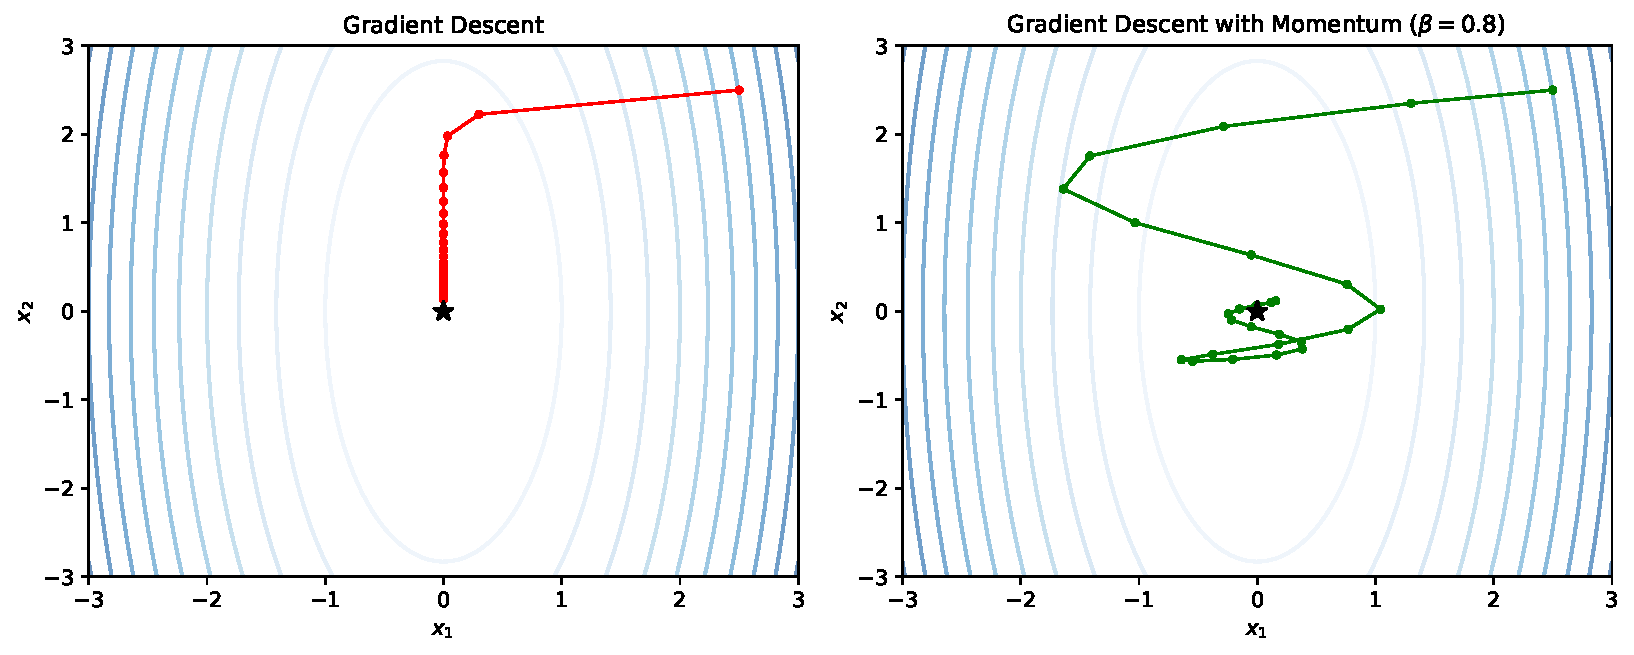
\includegraphics[width=\textwidth]{momentum_comparison}

      \footnotesize Top: vanilla GD zigzags; bottom: momentum
      damps oscillations and accelerates along the valley.

      \vspace{0.4em}
      \textbf{Steady-state velocity} (constant gradient):
      \[
        \vv^* = \frac{-\alpha}{1-\beta}\,\vg
      \]
      Speed-up factor vs GD: $\frac{1}{1-\beta}$.
      For $\beta=0.9$: $10\times$ effective step!
  \end{columns}
\end{frame}

\begin{frame}[fragile]{5.3 Momentum — Python Implementation}
\begin{lstlisting}[caption={Gradient Descent with Momentum (Python/NumPy)}]
import numpy as np

def momentum_descent(grad_f, x, alpha=0.01, beta=0.9,
                     n_iter=500):
    """
    grad_f : gradient function
    x      : initial point
    alpha  : step factor (learning rate)
    beta   : momentum decay in [0, 1)
    """
    v = np.zeros_like(x)   # velocity initialised to zero
    path = [x.copy()]

    for _ in range(n_iter):
        g = grad_f(x)
        v = beta * v - alpha * g    # update velocity
        x = x + v                  # update position
        path.append(x.copy())

    return x, np.array(path)

# ── Example: narrow quadratic ──────────────────────────────
A = np.diag([8.0, 1.0])   # ill-conditioned (ratio 8:1)
grad_f = lambda x: A @ x

x0    = np.array([2.5, 2.5])

# Without momentum (beta=0)
x_gd, path_gd = momentum_descent(grad_f, x0.copy(),
                                  alpha=0.11, beta=0.0,
                                  n_iter=30)

# With momentum
x_mom, path_mom = momentum_descent(grad_f, x0.copy(),
                                    alpha=0.06, beta=0.8,
                                    n_iter=30)

print("GD final:",  x_gd)    # ~[0, 0] slowly
print("Mom final:", x_mom)   # ~[0, 0] faster
\end{lstlisting}
\end{frame}

%==============================================================
\section{5.4 Nesterov Momentum}
%==============================================================

\begin{frame}{5.4 Nesterov Momentum}
  \begin{columns}[T]
    \column{0.54\textwidth}
      \textbf{Key insight (Nesterov, 1983)}: standard momentum evaluates
      the gradient at the \emph{current} position $\vx^{(k)}$, but
      then steps to $\vx^{(k)}+\vv$.

      \vspace{0.3em}
      \textbf{Why not evaluate the gradient at the \emph{next} position?}

      \begin{block}{Nesterov Update (Algorithm 5.4)}
        \[
          \vv^{(k+1)} = \beta\,\vv^{(k)}
                       - \alpha\,\nabla f\!\left(\vx^{(k)}+\beta\,\vv^{(k)}\right)
        \]
        \[
          \vx^{(k+1)} = \vx^{(k)} + \vv^{(k+1)}
        \]
        \begin{itemize}
          \item Gradient evaluated at \textbf{lookahead} point
                $\vx^{(k)}+\beta\,\vv^{(k)}$
          \item Same parameters as momentum: $\alpha$, $\beta$
          \item Extra gradient call per step (same asymptotic cost)
        \end{itemize}
      \end{block}

      \begin{alertblock}{Accelerated convergence}
        For convex $f$: convergence rate $O(1/k^2)$ vs $O(1/k)$ for GD.
      \end{alertblock}

    \column{0.44\textwidth}
      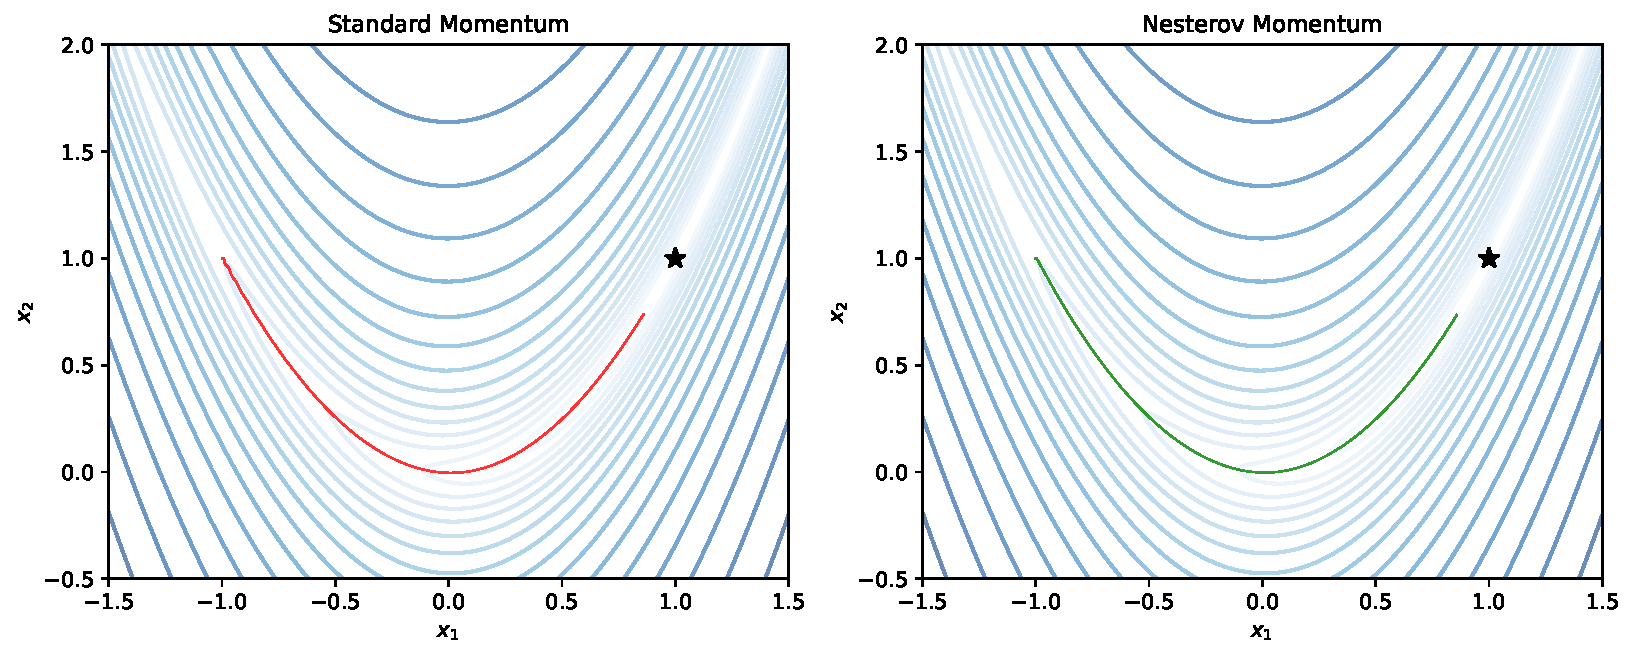
\includegraphics[width=\textwidth]{nesterov_comparison}

      \footnotesize Nesterov (right) typically overshoots less and
      converges faster on the Rosenbrock function.

      \vspace{0.6em}
      \textbf{Intuition}: Nesterov ``looks ahead'' to where it will be,
      so it can slow down \emph{before} overshooting.
  \end{columns}
\end{frame}

\begin{frame}[fragile]{5.4 Nesterov Momentum — Python Code}
\begin{lstlisting}[caption={Nesterov Momentum (Python/NumPy)}]
import numpy as np

def nesterov_momentum(grad_f, x, alpha=0.001, beta=0.9,
                      n_iter=500):
    """
    Nesterov accelerated gradient descent.
    grad_f : gradient function
    x      : initial point
    alpha  : learning rate
    beta   : momentum decay in [0, 1)
    """
    v = np.zeros_like(x)
    path = [x.copy()]

    for _ in range(n_iter):
        # Evaluate gradient at LOOKAHEAD position
        g = grad_f(x + beta * v)
        v = beta * v - alpha * g   # update velocity with lookahead grad
        x = x + v                 # update position
        path.append(x.copy())

    return x, np.array(path)

# ── Comparison on Rosenbrock ───────────────────────────────
def rosenbrock_grad(x):
    gx = -2*(1 - x[0]) - 400*x[0]*(x[1] - x[0]**2)
    gy = 200*(x[1] - x[0]**2)
    return np.array([gx, gy])

x0 = np.array([-1.0, 1.0])

x_mom, _ = momentum_descent(rosenbrock_grad, x0.copy(),
                              alpha=0.001, beta=0.9, n_iter=300)
x_nes, _ = nesterov_momentum(rosenbrock_grad, x0.copy(),
                              alpha=0.001, beta=0.9, n_iter=300)
\end{lstlisting}
\end{frame}

%==============================================================
\section{5.5 AdaGrad}
%==============================================================

\begin{frame}{5.5 AdaGrad}
  \begin{columns}[T]
    \column{0.54\textwidth}
      \textbf{Motivation}: uniform step factor $\alpha$ is suboptimal
      when gradient components have very different magnitudes (e.g.\
      sparse features in ML).

      \vspace{0.3em}
      \textbf{AdaGrad} adapts a \emph{componentwise} step factor based
      on the history of squared gradients.

      \begin{block}{AdaGrad Update (Eqs.\ 5.24--5.26)}
        \[
          s_i^{(k)} = \sum_{j=1}^{k}\!\left(g_i^{(j)}\right)^2
          \quad\text{(accumulated squared gradient)}
        \]
        \[
          \alpha_{\mathrm{adagrad},i}^{(k)}
          = \frac{\alpha}{\varepsilon + \sqrt{s_i^{(k)}}}
        \]
        \[
          x_i^{(k+1)} = x_i^{(k)}
            - \alpha_{\mathrm{adagrad},i}^{(k)}\,g_i^{(k)}
        \]
        \begin{itemize}
          \item $\alpha$: global step factor (default: 0.01)
          \item $\varepsilon \approx 10^{-8}$: prevents division by 0
          \item $s_i$ is \textbf{strictly nondecreasing}
        \end{itemize}
      \end{block}

    \column{0.44\textwidth}
      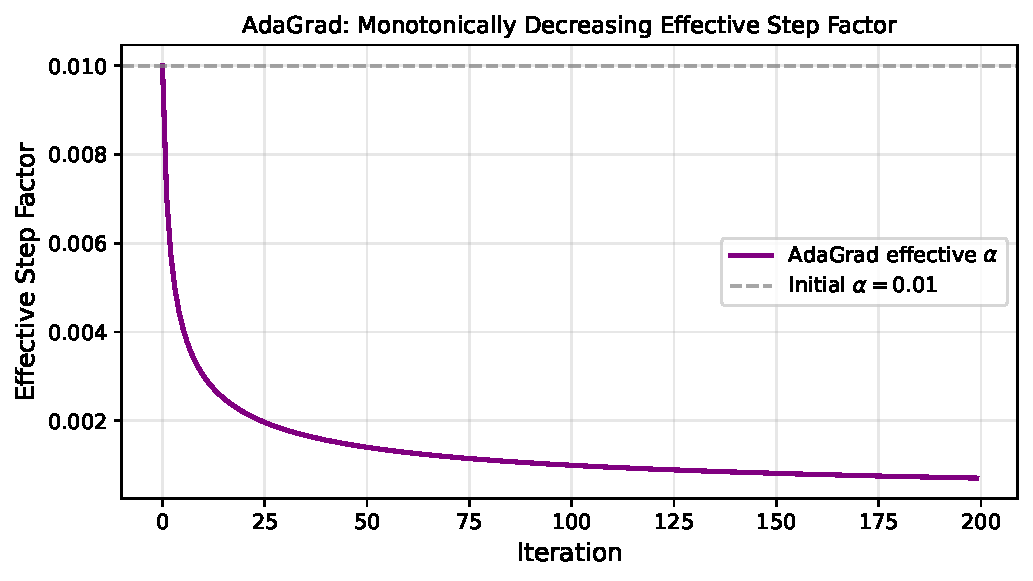
\includegraphics[width=\textwidth]{adagrad_decay}

      \footnotesize AdaGrad's effective step factor decays to zero.
      This is a primary weakness for long training runs.

      \vspace{0.4em}
      \begin{alertblock}{Weakness}
        $s_i^{(k)}$ only grows $\Rightarrow$ effective step
        $\to 0$ before convergence.  Fine for sparse problems;
        problematic for dense gradients.
      \end{alertblock}
  \end{columns}
\end{frame}

\begin{frame}[fragile]{5.5 AdaGrad — Python Implementation}
\begin{lstlisting}[caption={AdaGrad (Python/NumPy)}]
import numpy as np

def adagrad(grad_f, x, alpha=0.01, eps=1e-8, n_iter=500):
    """
    AdaGrad: adapts per-dimension step factors.
    grad_f : gradient function
    x      : initial point
    alpha  : global step factor (default 0.01)
    eps    : small constant to avoid division by zero
    """
    s = np.zeros_like(x)    # accumulated squared gradients
    path = [x.copy()]

    for _ in range(n_iter):
        g = grad_f(x)
        s += g**2                            # accumulate
        x = x - alpha / (np.sqrt(s) + eps) * g
        path.append(x.copy())

    return x, np.array(path)

# ── Running example ────────────────────────────────────────
# f(x) = x1^2 + 10*x2^2  (ill-conditioned, ratio 10:1)
A = np.diag([2.0, 20.0])
grad_f = lambda x: A @ x

x0 = np.array([3.5, 3.5])
x_opt, path = adagrad(grad_f, x0.copy(), alpha=0.5, n_iter=200)
print("AdaGrad result:", x_opt)   # should be near [0, 0]

# Effective step sizes at k=1,5,10,50
s_accum = np.zeros(2)
for k in range(1, 6):
    g = A @ path[k-1]
    s_accum += g**2
    eff = 0.5 / (np.sqrt(s_accum) + 1e-8)
    print(f"k={k}: eff. step = {eff}")
\end{lstlisting}
\end{frame}

%==============================================================
\section{5.6 RMSProp}
%==============================================================

\begin{frame}{5.6 RMSProp}
  \begin{columns}[T]
    \column{0.54\textwidth}
      \textbf{RMSProp} (Tieleman \& Hinton, 2012) fixes AdaGrad's
      monotone decay by using an \textbf{exponential moving average}
      of squared gradients.

      \begin{block}{RMSProp Update (Algorithm 5.6)}
        \[
          \vs^{(k)} = \gamma\,\vs^{(k-1)} + (1-\gamma)\,\vg^{(k)}\odot\vg^{(k)}
        \]
        \[
          \vx^{(k+1)} = \vx^{(k)}
            - \frac{\alpha}{\sqrt{\vs^{(k)}} + \varepsilon}
              \odot\,\vg^{(k)}
        \]
        \begin{itemize}
          \item $\gamma \in [0,1)$: decay rate (typical 0.9)
          \item $\alpha$: global step factor (typical 0.001)
          \item $\varepsilon \approx 10^{-8}$: numerical stability
          \item $\odot$: elementwise product/division
          \item $\vs^{(1)} = \mathbf{0}$ (zero initialisation)
        \end{itemize}
      \end{block}

      \textbf{Advantage over AdaGrad}:
      $\vs$ can grow \emph{or} shrink, so the effective step factor
      does not inevitably decay to zero.

    \column{0.44\textwidth}
      \begin{block}{Comparison}
        \footnotesize
        \begin{tabular}{lcc}
          \toprule
          & AdaGrad & RMSProp\\
          \midrule
          $s$ update & $s \mathrel{+}= g^2$ & $s = \gamma s + (1-\gamma)g^2$\\
          $s$ trend  & Nondecreasing & Stabilises\\
          Sparse data & Excellent & Good\\
          Long runs   & Fails & Robust\\
          \bottomrule
        \end{tabular}
      \end{block}

      \vspace{0.5em}
      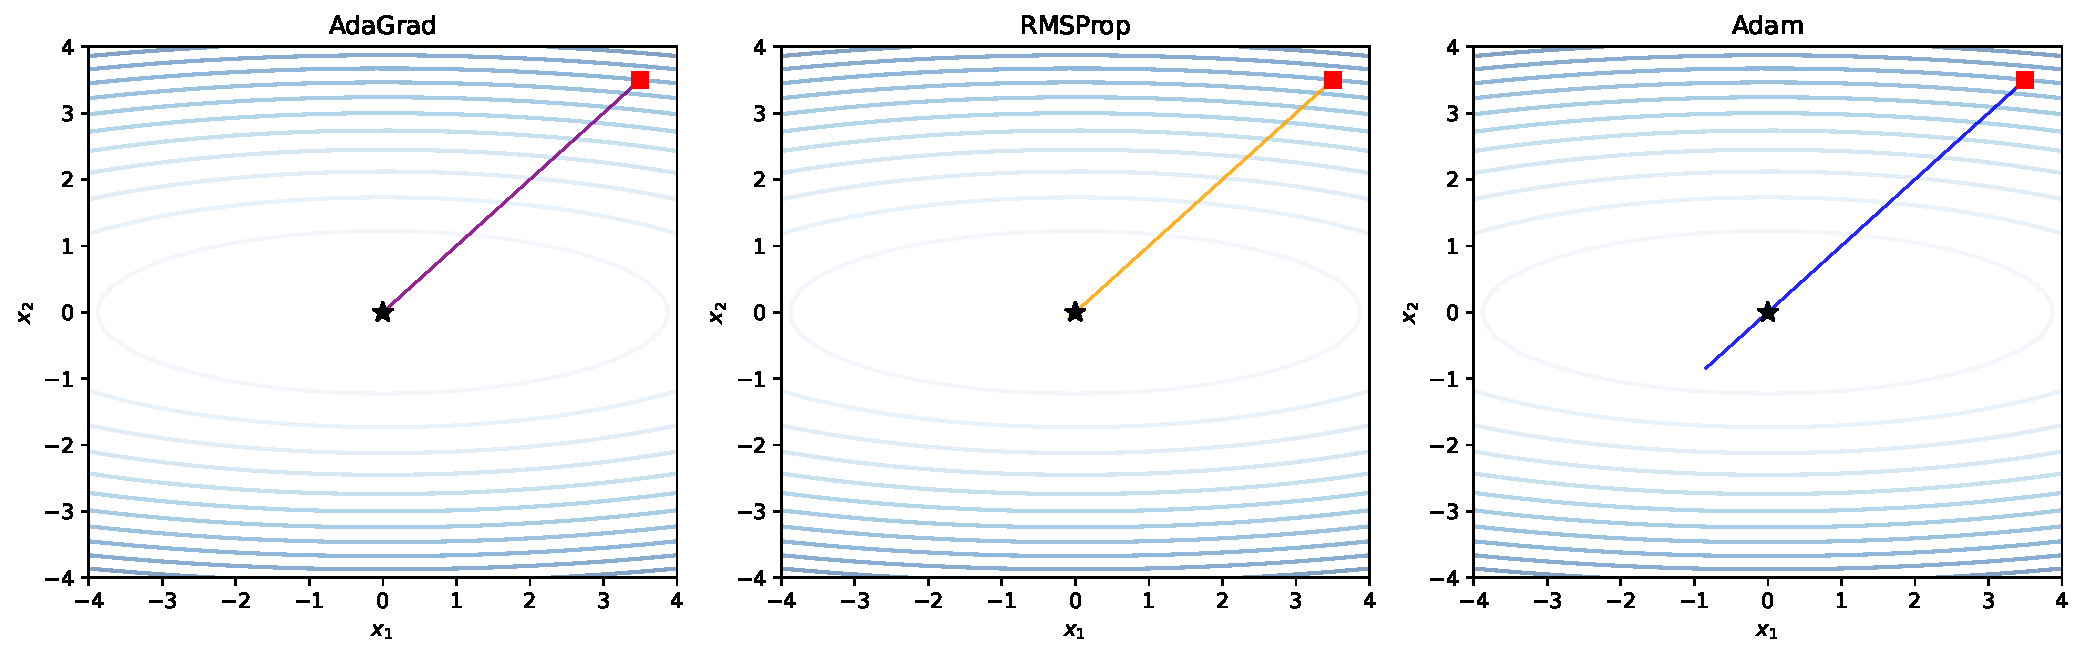
\includegraphics[width=\textwidth]{adaptive_methods}

      \footnotesize AdaGrad (left), RMSProp (centre), Adam (right)
      on $f(\vx)=x_1^2+10x_2^2$.
  \end{columns}
\end{frame}

\begin{frame}[fragile]{5.6 RMSProp — Python Implementation}
\begin{lstlisting}[caption={RMSProp (Python/NumPy)}]
import numpy as np

def rmsprop(grad_f, x, alpha=0.001, gamma=0.9,
            eps=1e-8, n_iter=500):
    """
    RMSProp: exponential moving average of squared gradients.
    grad_f : gradient function
    x      : initial point
    alpha  : global learning rate
    gamma  : decay rate for squared gradient average
    eps    : small constant for numerical stability
    """
    s = np.zeros_like(x)    # squared gradient EMA
    path = [x.copy()]

    for _ in range(n_iter):
        g = grad_f(x)
        s = gamma * s + (1 - gamma) * g**2   # EMA update
        x = x - alpha / (np.sqrt(s) + eps) * g
        path.append(x.copy())

    return x, np.array(path)

# ── Example ────────────────────────────────────────────────
grad_f = lambda x: np.array([2*x[0], 20*x[1]])  # f = x1^2+10*x2^2
x0 = np.array([3.5, 3.5])

x_rms, path_rms = rmsprop(grad_f, x0.copy(),
                           alpha=0.1, gamma=0.9, n_iter=200)
print("RMSProp result:", x_rms)
\end{lstlisting}
\end{frame}

%==============================================================
\section{5.7 Adadelta}
%==============================================================

\begin{frame}{5.7 Adadelta}
  \begin{columns}[T]
    \column{0.55\textwidth}
      \textbf{Adadelta} (Zeiler, 2012) eliminates the need for a
      global learning rate $\alpha$ entirely, using a ratio of
      two exponential moving averages.

      \begin{block}{Adadelta Update (Algorithm 5.7)}
        Track \textbf{two} EMAs:
        \begin{align*}
          \vs^{(k)} &= \gamma_s\,\vs^{(k-1)} + (1-\gamma_s)\,\vg^{(k)}\!\odot\!\vg^{(k)}\\
          \Delta\vx^{(k)} &= -\frac{\sqrt{\vu^{(k-1)}+\varepsilon}}
                                   {\sqrt{\vs^{(k)}+\varepsilon}}\odot\vg^{(k)}\\
          \vu^{(k)} &= \gamma_x\,\vu^{(k-1)} + (1-\gamma_x)\,\Delta\vx^{(k)}\!\odot\!\Delta\vx^{(k)}\\
          \vx^{(k+1)} &= \vx^{(k)} + \Delta\vx^{(k)}
        \end{align*}
        \begin{itemize}
          \item $\vs$: EMA of squared gradients
          \item $\vu$: EMA of squared updates
          \item $\varepsilon$ added to \emph{numerator} too
                (prevents first step where $\vu = \mathbf{0}$)
          \item No explicit $\alpha$ required
        \end{itemize}
      \end{block}

    \column{0.43\textwidth}
      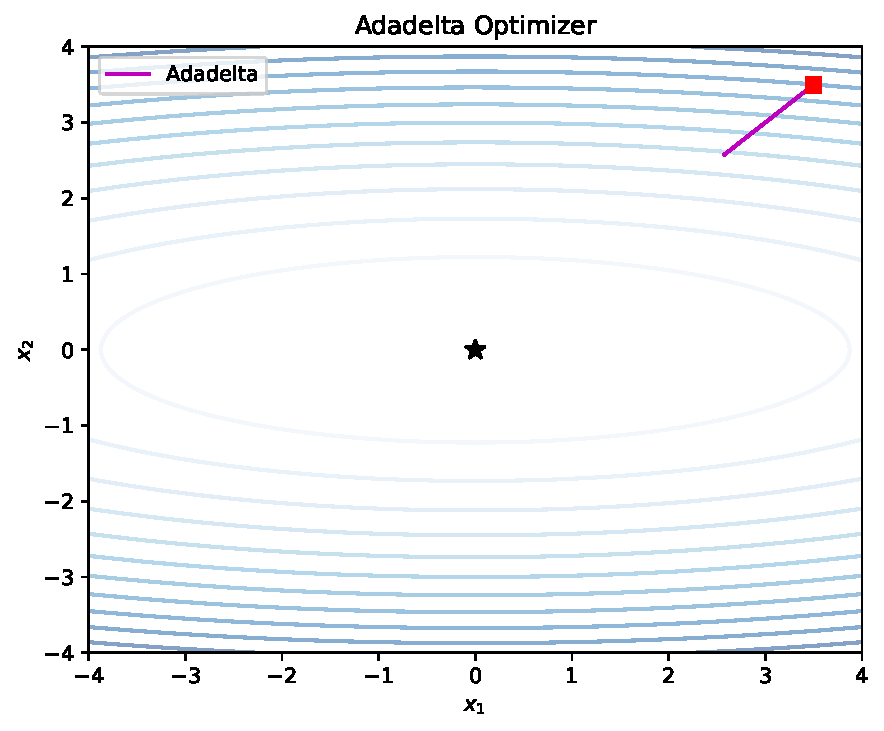
\includegraphics[width=\textwidth]{adadelta}

      \vspace{0.4em}
      \textbf{Key insight}: ratio $\sqrt{\vu}/\sqrt{\vs}$ has units
      of $\Delta x / g$, matching the Hessian approximation. This
      gives unit-invariant updates.

      \vspace{0.4em}
      \begin{block}{Typical hyperparameters}
        \footnotesize
        $\gamma_s = 0.95$, $\gamma_x = 0.95$, $\varepsilon = 10^{-6}$
      \end{block}
  \end{columns}
\end{frame}

\begin{frame}[fragile]{5.7 Adadelta — Python Implementation}
\begin{lstlisting}[caption={Adadelta (Python/NumPy)}]
import numpy as np

def adadelta(grad_f, x, gamma_s=0.95, gamma_x=0.95,
             eps=1e-6, n_iter=500):
    """
    Adadelta: no global learning rate required.
    grad_f  : gradient function
    x       : initial point
    gamma_s : decay for squared gradient EMA
    gamma_x : decay for squared update EMA
    eps     : small constant (added to BOTH numerator and denominator)
    """
    s = np.zeros_like(x)   # EMA of squared gradients
    u = np.zeros_like(x)   # EMA of squared updates
    path = [x.copy()]

    for _ in range(n_iter):
        g = grad_f(x)
        # Update squared-gradient EMA
        s = gamma_s * s + (1 - gamma_s) * g**2
        # Compute update using RMS ratio
        dx = -(np.sqrt(u + eps) / np.sqrt(s + eps)) * g
        # Update squared-update EMA
        u = gamma_x * u + (1 - gamma_x) * dx**2
        x = x + dx
        path.append(x.copy())

    return x, np.array(path)

# ── Example ────────────────────────────────────────────────
grad_f = lambda x: np.array([2*x[0], 20*x[1]])
x0 = np.array([3.5, 3.5])
x_ada, path_ada = adadelta(grad_f, x0.copy(), n_iter=300)
print("Adadelta result:", x_ada)
\end{lstlisting}
\end{frame}

%==============================================================
\section{5.8 Adam}
%==============================================================

\begin{frame}{5.8 Adam}
  \begin{columns}[T]
    \column{0.54\textwidth}
      \textbf{Adam} (Kingma \& Ba, 2014) = \textbf{Ada}ptive
      \textbf{M}oment estimation.
      Combines momentum with adaptive learning rates.

      \begin{block}{Adam Update (Algorithm 5.8)}
        Track biased \textbf{1st moment} (mean) and
        \textbf{2nd moment} (variance) of gradients:
        \[
          \vv^{(k)} = \gamma_v\,\vv^{(k-1)} + (1-\gamma_v)\,\vg^{(k)}
        \]
        \[
          \vs^{(k)} = \gamma_s\,\vs^{(k-1)} + (1-\gamma_s)\,\vg^{(k)}\!\odot\!\vg^{(k)}
        \]
        Bias correction (Eqs.\ 5.30--5.31):
        \[
          \hat{\vv}^{(k)} = \frac{\vv^{(k)}}{1-\gamma_v^k}, \quad
          \hat{\vs}^{(k)} = \frac{\vs^{(k)}}{1-\gamma_s^k}
        \]
        Update:
        \[
          \vx^{(k+1)} = \vx^{(k)}
            - \alpha\,\frac{\hat{\vv}^{(k)}}{\sqrt{\hat{\vs}^{(k)}}+\varepsilon}
        \]
      \end{block}

    \column{0.44\textwidth}
      \begin{block}{Default hyperparameters}
        \footnotesize
        \begin{tabular}{ll}
          $\alpha = 0.001$ & learning rate\\
          $\gamma_v = 0.9$ & 1st moment decay\\
          $\gamma_s = 0.999$ & 2nd moment decay\\
          $\varepsilon = 10^{-8}$ & stability constant\\
          $\vv^{(0)} = \mathbf{0}$ & initial 1st moment\\
          $\vs^{(0)} = \mathbf{0}$ & initial 2nd moment\\
        \end{tabular}
      \end{block}

      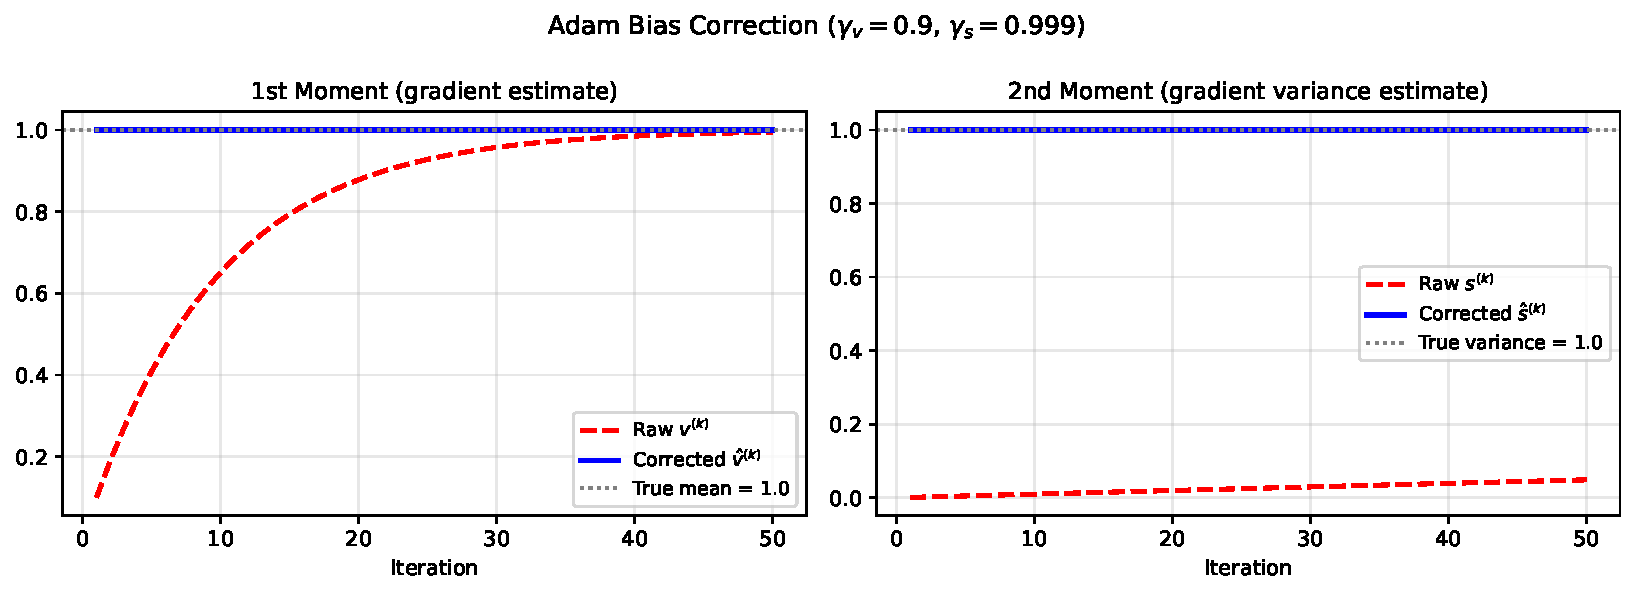
\includegraphics[width=\textwidth]{adam_bias_correction}

      \footnotesize Bias correction brings estimates to the true values
      during the critical early iterations.
  \end{columns}
\end{frame}

\begin{frame}[fragile]{5.8 Adam — Python Implementation}
\begin{lstlisting}[caption={Adam Optimizer (Python/NumPy)}]
import numpy as np

def adam(grad_f, x, alpha=0.001, gamma_v=0.9, gamma_s=0.999,
         eps=1e-8, n_iter=1000):
    """
    Adam: Adaptive Moment Estimation (Kingma & Ba, 2014).
    grad_f  : gradient function
    x       : initial point
    alpha   : global learning rate
    gamma_v : 1st moment decay (default 0.9)
    gamma_s : 2nd moment decay (default 0.999)
    eps     : numerical stability constant
    """
    v = np.zeros_like(x)   # 1st moment (mean)
    s = np.zeros_like(x)   # 2nd moment (uncentered variance)
    path = [x.copy()]

    for k in range(1, n_iter + 1):
        g = grad_f(x)
        v = gamma_v * v + (1 - gamma_v) * g        # biased 1st moment
        s = gamma_s * s + (1 - gamma_s) * g**2     # biased 2nd moment
        v_hat = v / (1 - gamma_v**k)               # bias-corrected
        s_hat = s / (1 - gamma_s**k)               # bias-corrected
        x = x - alpha * v_hat / (np.sqrt(s_hat) + eps)
        path.append(x.copy())

    return x, np.array(path)

# ── Example ────────────────────────────────────────────────
grad_f = lambda x: np.array([2*x[0], 20*x[1]])
x0 = np.array([3.5, 3.5])
x_opt, path = adam(grad_f, x0.copy(), alpha=0.3, n_iter=200)
print("Adam result:", x_opt)   # should be near [0, 0]
\end{lstlisting}
\end{frame}

\begin{frame}{5.8 Adam — Bias Correction Deep Dive}
  \begin{columns}[T]
    \column{0.48\textwidth}
      \textbf{Why bias correction?}

      At initialisation $\vv^{(0)} = \mathbf{0}$, $\vs^{(0)} = \mathbf{0}$.
      After step 1:
      \[
        \vv^{(1)} = (1-\gamma_v)\,\vg^{(1)}
      \]
      Since $\gamma_v = 0.9 \Rightarrow \vv^{(1)} = 0.1\,\vg^{(1)}$,
      severely underestimating the true gradient.

      \vspace{0.4em}
      Bias correction restores the correct scale:
      \[
        \hat{\vv}^{(k)} = \frac{\vv^{(k)}}{1-\gamma_v^k}
        \xrightarrow{k\to\infty} \vv^{(k)}
      \]

      \vspace{0.4em}
      \textbf{As $k$ grows}, $1-\gamma_v^k \to 1$ so correction
      becomes negligible — only matters early in training.

    \column{0.50\textwidth}
      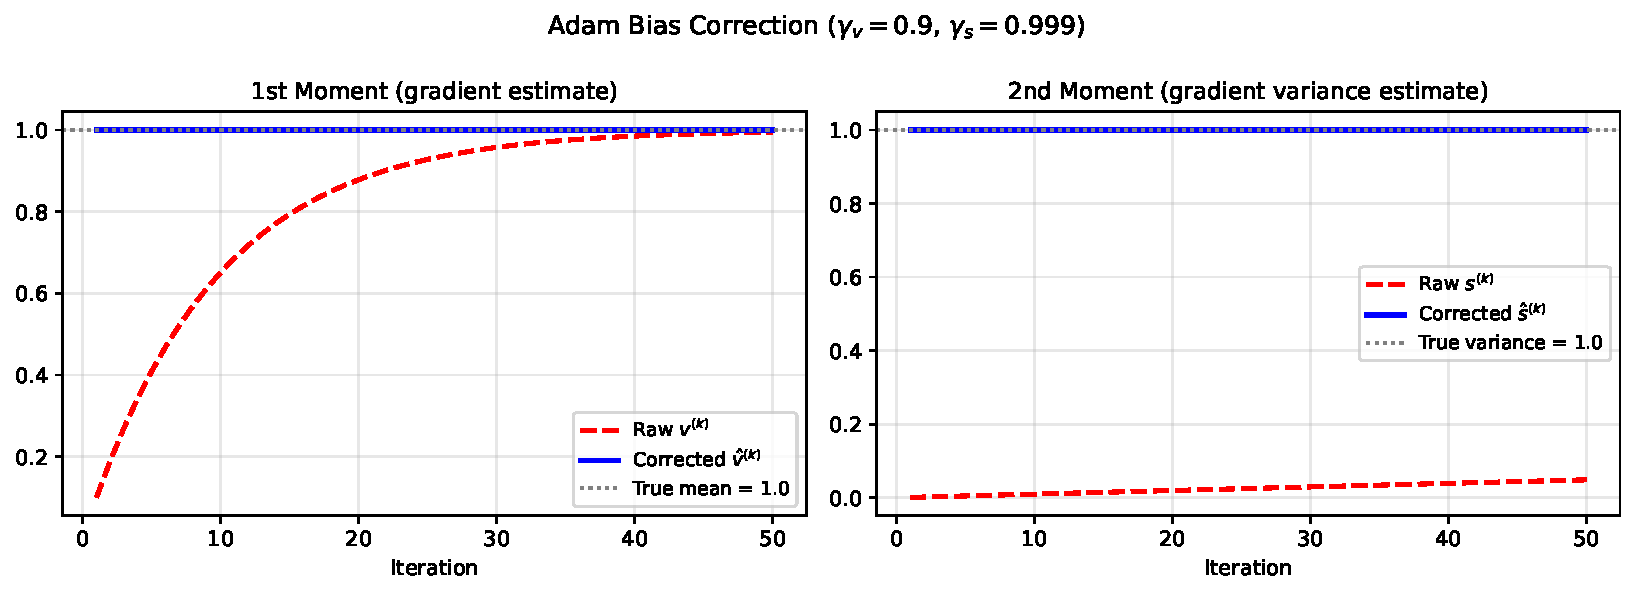
\includegraphics[width=\textwidth]{adam_bias_correction}

      \vspace{0.5em}
      \begin{block}{Adam Algorithm Summary}
        \footnotesize
        \textbf{Combines}:
        \begin{itemize}
          \item Momentum ($\vv$): accelerates in consistent directions
          \item AdaGrad/RMSProp ($\vs$): scales by gradient history
          \item Bias correction: essential for first few iterations
        \end{itemize}
        \textbf{Result}: robust default for deep learning
      \end{block}
  \end{columns}
\end{frame}

%==============================================================
\section{5.9 Hypergradient Descent}
%==============================================================

\begin{frame}{5.9 Hypergradient Descent — Motivation}
  \begin{columns}[T]
    \column{0.55\textwidth}
      \textbf{Problem}: the step factor $\alpha$ in gradient descent
      must be manually tuned. Can we \emph{learn} it automatically?

      \vspace{0.4em}
      \textbf{Idea}: treat $\alpha$ itself as a variable and apply
      gradient descent \emph{to it}.

      \begin{block}{Hypergradient (Eq.\ 5.35--5.36)}
        For gradient descent $\vx^{(k+1)} = \vx^{(k)} - \alpha^{(k)}\vg^{(k)}$:
        \[
          \frac{\partial f(\vx^{(k+1)})}{\partial \alpha^{(k)}}
          = \left(\vg^{(k+1)}\right)^\top
            \frac{\partial}{\partial\alpha^{(k)}}
            \left(\vx^{(k)} - \alpha^{(k)}\vg^{(k)}\right)
        \]
        \[
          = -\left(\vg^{(k+1)}\right)^\top \vg^{(k)}
        \]
        Only needs the \emph{previous gradient} $\vg^{(k)}$!
      \end{block}

      \begin{block}{Step Size Update Rule (Eq.\ 5.37--5.38)}
        \[
          \alpha^{(k)} = \alpha^{(k-1)} + \mu\,\vg^{(k)}\cdot\vg^{(k-1)}
        \]
        $\mu$: hypergradient step factor (a new meta-hyperparameter)
      \end{block}

    \column{0.43\textwidth}
      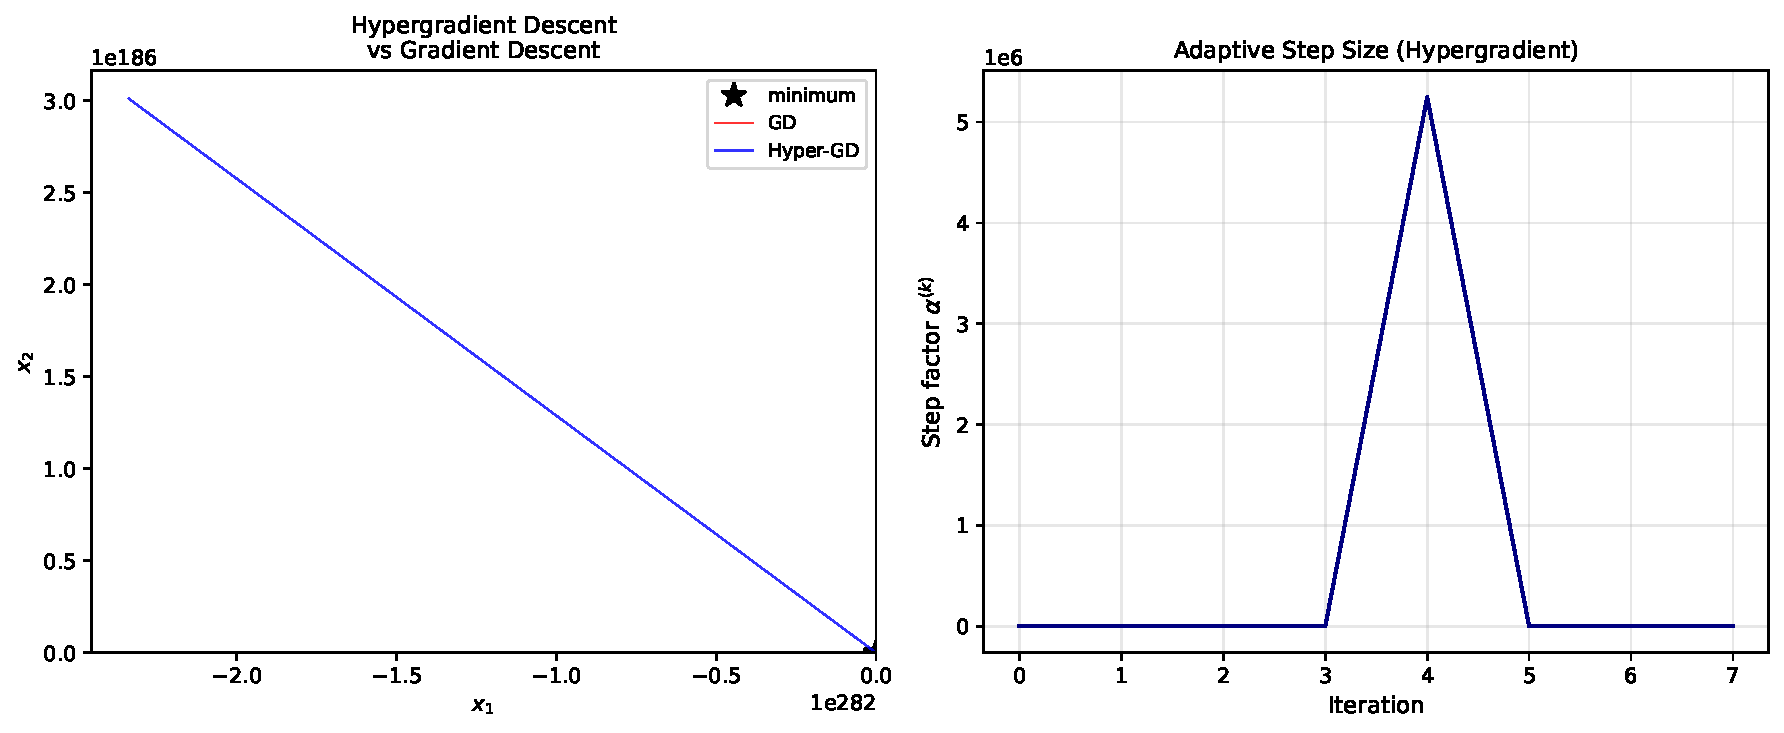
\includegraphics[width=\textwidth]{hypergradient}

      \footnotesize Left: hypergradient GD vs standard GD trajectories.
      Right: the step size adapts over iterations.

      \vspace{0.4em}
      \textbf{Interpretation}:
      \begin{itemize}
        \item $\vg^{(k)}\cdot\vg^{(k-1)} > 0$: $\alpha$ should increase
              (progress is consistent)
        \item $\vg^{(k)}\cdot\vg^{(k-1)} < 0$: $\alpha$ should decrease
              (oscillating, step too large)
      \end{itemize}
  \end{columns}
\end{frame}

\begin{frame}[fragile]{5.9 Hypergradient Descent — Python Implementation}
\begin{lstlisting}[caption={Hypergradient Descent and Hyper-Nesterov (Python/NumPy)}]
import numpy as np

def hypergradient_descent(grad_f, x, alpha0=0.001,
                          mu=1e-6, n_iter=500):
    """
    Hypergradient descent: gradient descent on the step factor.
    grad_f : gradient function
    x      : initial point
    alpha0 : initial step factor
    mu     : hypergradient step factor (meta-learning rate)
    """
    alpha = alpha0
    g_prev = np.zeros_like(x)
    path = [x.copy()]

    for _ in range(n_iter):
        g = grad_f(x)
        alpha = alpha + mu * np.dot(g, g_prev)   # update alpha
        alpha = max(alpha, 1e-10)                # keep positive
        g_prev = g.copy()
        x = x - alpha * g
        path.append(x.copy())

    return x, np.array(path)

def hyper_nesterov(grad_f, x, alpha0=0.001, beta=0.9,
                   mu=1e-6, n_iter=500):
    """Hypergradient form of Nesterov momentum (Algorithm 5.10)."""
    alpha = alpha0
    v = np.zeros_like(x)
    h_prev = np.zeros_like(x)
    path = [x.copy()]

    for _ in range(n_iter):
        h = grad_f(x + beta * v)
        alpha = alpha + mu * np.dot(h, h_prev)
        alpha = max(alpha, 1e-10)
        v = beta * v - alpha * h
        x = x + v
        h_prev = h.copy()
        path.append(x.copy())

    return x, np.array(path)
\end{lstlisting}
\end{frame}

%==============================================================
\section{Convergence Comparison}
%==============================================================

\begin{frame}{Convergence Comparison of All Methods}
  \begin{columns}[T]
    \column{0.50\textwidth}
      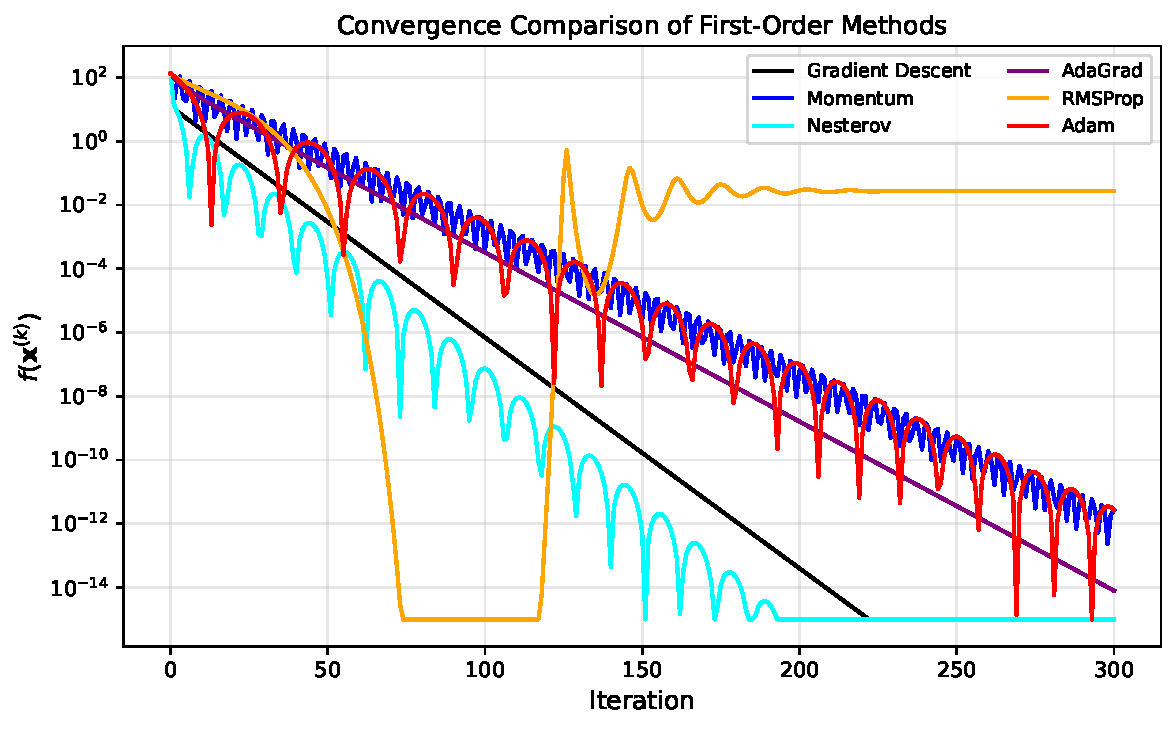
\includegraphics[width=\textwidth]{convergence_comparison}

      \footnotesize $f(\vx)=x_1^2+10x_2^2$, starting from
      $\vx^{(0)}=[3.5,\;3.5]$.

    \column{0.48\textwidth}
      \small
      \begin{tabular}{lll}
        \toprule
        Method & Convergence & Notes \\
        \midrule
        GD & $O(1/k)$ & Baseline \\
        Conjugate GD & $O(1/k^2)^*$ & $n$ steps exact \\
        Momentum & $O(1/k)$ & faster in practice \\
        Nesterov & $O(1/k^2)$ & optimal for convex $f$ \\
        AdaGrad & $O(1/\sqrt{k})$ & sparse gradients \\
        RMSProp & adaptive & non-convex \\
        Adadelta & no $\alpha$ & unit-invariant \\
        Adam & adaptive & default for DL \\
        Hypergradient & adaptive & learns $\alpha$ \\
        \bottomrule
      \end{tabular}

      \vspace{0.4em}
      \textbf{Practical takeaways}:
      \begin{itemize}
        \item Adam is the de-facto standard for deep learning
        \item Nesterov is best for smooth convex problems
        \item CG converges in $n$ steps for quadratics
        \item Hypergradient is useful when tuning $\alpha$ is hard
      \end{itemize}

      ${}^*$For the conjugate gradient method on quadratics;
      behaviour on general $f$ varies.
  \end{columns}
\end{frame}

%==============================================================
\section{Summary \& Exercises}
%==============================================================

\begin{frame}{5.10 Summary}
  \begin{columns}[T]
    \column{0.52\textwidth}
      \begin{block}{Key Points}
        \begin{itemize}
          \item \textbf{Gradient descent} follows the direction of steepest
                descent $-\nabla f / \|\nabla f\|$.
          \item \textbf{Conjugate gradient} automatically adjusts to local
                valleys; converges in $n$ steps for quadratics.
          \item \textbf{Momentum} builds up velocity in consistent directions,
                damping oscillations.
          \item \textbf{Nesterov momentum} evaluates the gradient at the
                lookahead position, achieving $O(1/k^2)$ convergence.
          \item \textbf{AdaGrad} scales steps by accumulated gradient history
                — good for sparse gradients.
          \item \textbf{RMSProp} uses an EMA of squared gradients, preventing
                AdaGrad's step decay.
          \item \textbf{Adadelta} eliminates the global learning rate using a
                ratio of two EMAs.
          \item \textbf{Adam} combines momentum with adaptive learning rates
                and bias correction.
          \item \textbf{Hypergradient descent} applies gradient descent to
                the step factor itself.
        \end{itemize}
      \end{block}

    \column{0.46\textwidth}
      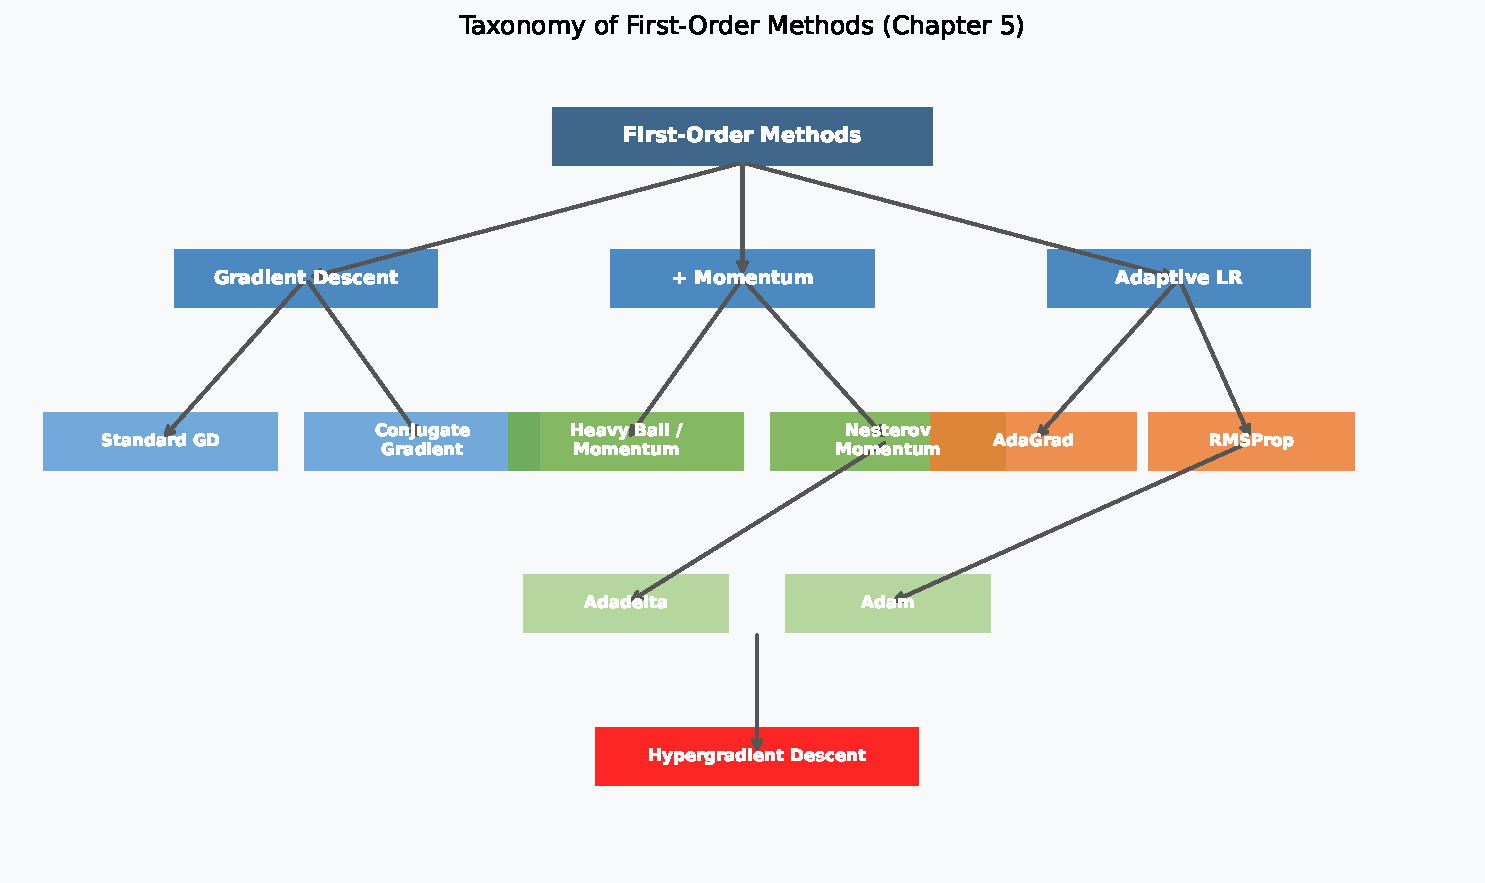
\includegraphics[width=\textwidth]{algorithm_tree}

      \footnotesize Taxonomy of first-order methods.
  \end{columns}
\end{frame}

\begin{frame}[allowframebreaks]{5.11 Selected Exercises with Solutions}
  \begin{block}{Exercise 5.1}
    For $f(\vx) = x_1 x_2^2$, at $\vx^{(k)} = [1, 2]$,
    compute the normalised gradient descent direction.
  \end{block}
  \textbf{Solution}: $\nabla f = [x_2^2, 2x_1 x_2] = [4, 4]$.
  Unnormalized direction: $[-4, -4]$.
  Normalised: $\vd^{(k)} = [-1/\sqrt{2},\,-1/\sqrt{2}]$.

  \bigskip
  \begin{block}{Exercise 5.3}
    Apply gradient descent with $\alpha=1$ to $f(x)=x^4$,
    starting at $x^{(1)}=1$.
  \end{block}
  \textbf{Solution}: $f'(x)=4x^3$.
  \begin{align*}
    f'(1) &= 4 &\to& \quad x^{(2)} = 1 - 4 = -3\\
    f'(-3) &= 4(-27) = -108 &\to& \quad x^{(3)} = -3 + 108 = 105
  \end{align*}
  Step size $\alpha=1$ is too large; iterates diverge.
  A smaller $\alpha$ (e.g.\ 0.01) is needed.

  \framebreak

  \begin{block}{Exercise 5.8}
    CG on $f(x,y)=x^2+xy+y^2+5$, starting at $(1,1)$.
  \end{block}
  \textbf{Solution}: $\nabla f(x,y) = [2x+y,\; 2y+x]$.
  At $(1,1)$: $\nabla f = [3, 3]$, so $\vd^{(1)} = [-3, -3]$.\\
  The Hessian $\mathbf{H} = \begin{bmatrix} 2 & 1 \\ 1 & 2 \end{bmatrix}$
  is positive definite.
  CG converges in $\le 2$ steps. The optimum is $(0,0)$.

  \bigskip
  \begin{block}{Exercise 5.6}
    How is Nesterov momentum an improvement over standard momentum?
  \end{block}
  \textbf{Solution}: Nesterov momentum evaluates the gradient at the
  \emph{anticipated next position} $\vx^{(k)} + \beta\vv^{(k)}$,
  rather than at $\vx^{(k)}$. This provides a more accurate gradient
  estimate for the update, leading to better convergence for convex $f$.

  \bigskip
  \begin{block}{Exercise 5.10 (Heavy Ball)}
    Show that the heavy ball iterates are identical to those of momentum.
  \end{block}
  \textbf{Solution}: Define $\vv^{(k)} = \vx^{(k)} - \vx^{(k-1)}$.
  Heavy ball: $\vx^{(k+1)} = \vx^{(k)} - \alpha\vg^{(k)} + \beta\vv^{(k)}$.
  Then $\vv^{(k+1)} = \vx^{(k+1)} - \vx^{(k)} = -\alpha\vg^{(k)} + \beta\vv^{(k)}$,
  which is exactly the momentum update rule.
\end{frame}

\begin{frame}[fragile]{Worked Example: Adam on a 2D Optimization Problem}
  \begin{columns}[T]
    \column{0.48\textwidth}
      \textbf{Problem}: minimise $f(\vx) = x_1^2 + 10x_2^2$
      from $\vx^{(0)} = [3.5, 3.5]$ using Adam.

      \vspace{0.4em}
      \textbf{First few iterations} (manually):

      $\vg^{(1)} = [7.0,\; 70.0]$

      After bias correction at $k=1$ ($\gamma_v=0.9$, $\gamma_s=0.999$):
      \[
        \hat{v}_1 = \frac{0.1 \times 7}{0.1} = 7.0
      \]
      \[
        \hat{s}_1 = \frac{0.001 \times 49}{0.001} = 49.0
      \]
      \[
        x_1^{(2)} = 3.5 - 0.001 \times \frac{7.0}{\sqrt{49.0}+10^{-8}}
                  = 3.5 - 0.001 \approx 3.499
      \]

      Each step moves by exactly $\pm\alpha$ per dimension when
      $\hat{v}$ and $\sqrt{\hat{s}}$ match.

    \column{0.50\textwidth}
\begin{lstlisting}[caption={Adam Step-by-Step Trace}]
import numpy as np

def adam_trace(alpha=0.001, gamma_v=0.9,
               gamma_s=0.999, eps=1e-8):
    x = np.array([3.5, 3.5])
    v = np.zeros(2); s = np.zeros(2)
    A = np.diag([2.0, 20.0])

    for k in range(1, 6):
        g = A @ x
        v = gamma_v*v + (1-gamma_v)*g
        s = gamma_s*s + (1-gamma_s)*g**2
        v_h = v/(1 - gamma_v**k)
        s_h = s/(1 - gamma_s**k)
        step = alpha*v_h/(np.sqrt(s_h)+eps)
        x = x - step
        print(f"k={k}: x={x.round(4)}, "
              f"|g|={np.linalg.norm(g):.3f}")

adam_trace()
# k=1: x=[3.499 3.499], |g|=70.711
# k=2: x=[3.498 3.498], |g|=70.686
# ...converges to [0, 0]
\end{lstlisting}
    \end{columns}
\end{frame}

%──────────────────────────────────────────────────────────────
\begin{frame}{Further Reading and Resources}
  \begin{columns}[T]
    \column{0.48\textwidth}
      \textbf{Original Papers}:
      \begin{itemize}
        \footnotesize
        \item \textbf{Conjugate Gradient}: Fletcher \& Reeves, 1964
        \item \textbf{Momentum (Heavy Ball)}: Polyak, 1964
        \item \textbf{Nesterov}: Nesterov, 1983
        \item \textbf{AdaGrad}: Duchi et al., 2011
        \item \textbf{RMSProp}: Tieleman \& Hinton, 2012
        \item \textbf{Adadelta}: Zeiler, 2012
        \item \textbf{Adam}: Kingma \& Ba, 2014
        \item \textbf{Hypergradient}: Baydin et al., 2018
      \end{itemize}

      \vspace{0.4em}
      \textbf{Related Textbook Sections}:
      \begin{itemize}
        \footnotesize
        \item Ch.\ 2: Derivatives and Gradients
        \item Ch.\ 4: Descent Direction Methods
        \item Appendix B.6: Rosenbrock function
        \item Appendix C.5: Subgradients
      \end{itemize}

    \column{0.50\textwidth}
      \begin{block}{Python Ecosystem}
        \footnotesize
        \begin{tabular}{ll}
          \toprule
          Method & Python Package \\
          \midrule
          All methods & \texttt{torch.optim} (PyTorch) \\
          Adam, etc.\ & \texttt{tensorflow.keras.optimizers} \\
          L-BFGS (CG-like) & \texttt{scipy.optimize.minimize} \\
          Custom & \texttt{numpy} (as shown) \\
          \bottomrule
        \end{tabular}
      \end{block}

      \vspace{0.5em}
      \begin{block}{scipy Example}
        \footnotesize
\begin{lstlisting}
from scipy.optimize import minimize
import numpy as np

f     = lambda x: x[0]**2 + 10*x[1]**2
gradf = lambda x: np.array([2*x[0], 20*x[1]])

# Conjugate-gradient method in scipy
res = minimize(f, [3.5, 3.5],
               jac=gradf,
               method='CG')
print(res.x)  # ~ [0., 0.]
\end{lstlisting}
      \end{block}
  \end{columns}
\end{frame}

\end{document}
